\chapter{CFX Pre}
\label{ch:pre}

 Mesh specifications
 Boundary conditions
 Fluid properties
 Numerical parameters (discretization scheme), residual, max it, residuals, turbulence model)
 Computational domain justification 
 Applicability of $k-\varepsilon$ model


Computational domain in Figure~\ref{fig:domain}
\begin{figure}[H]
	\centering
	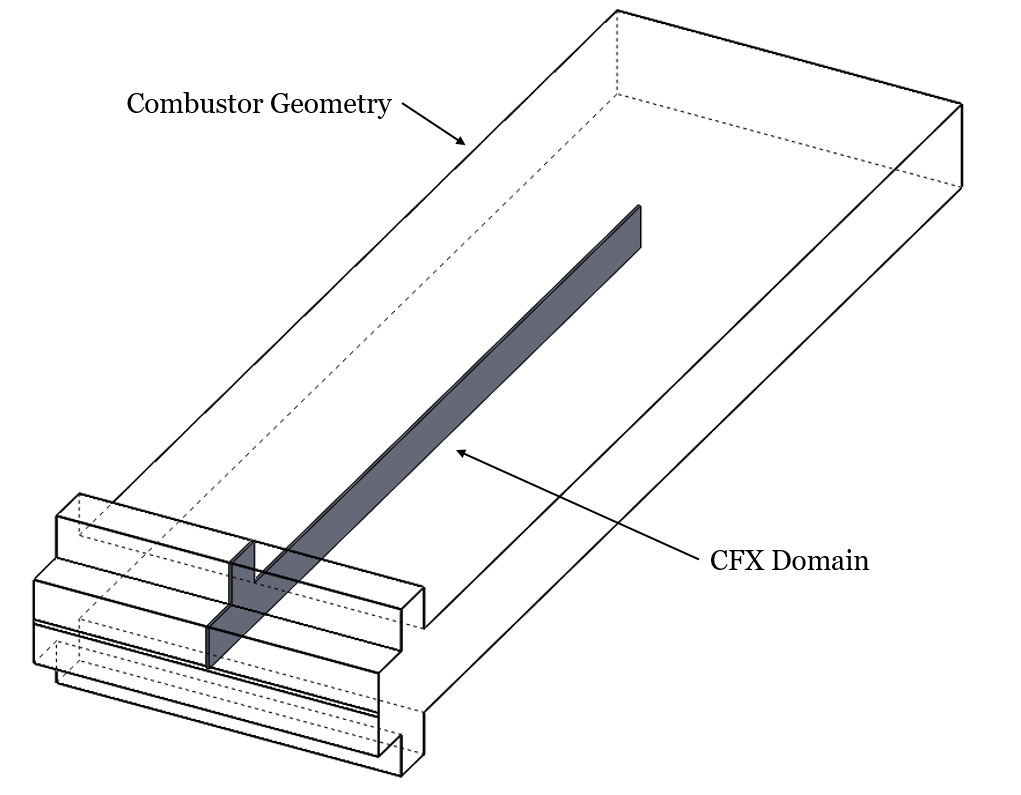
\includegraphics[scale=0.5]{ref/domain}
	\caption{Computational domain.}
	\label{fig:domain}
\end{figure}


%-----------------------------------------------------------------------------------------------------------------
\section{Mesh Specifications}
\label{sec:pre_mesh}

Summary of mesh



%-----------------------------------------------------------------------------------------------------------------
\section{Boundary Conditions}
\label{sec:pre_bc}

Summary of BC


%-----------------------------------------------------------------------------------------------------------------
\section{Fluid Properties}
\label{sec:pre_fluid}

Summary of fluid


%-----------------------------------------------------------------------------------------------------------------
\section{Numerical Parameters}
\label{sec:pre_num}

discretization	schemes, residual	target,	max	iterations,	turbulence mode


\begin{equation}
	\label{eq:ts}
	t_s = \frac{1}{3} \left( \frac{L_T}{U} \right)
\end{equation}

Using $L = L_d + X^* H = 285$ [mm] = 0.285 [m] $\Rightarrow \boldmath{t_s =}$ \textbf{0.004 [s]}.\\  

Thermal Energy (flow is not compressible hence don't use total) for heat transfer non buoyant.\\


Applicability of $k-\varepsilon$ Model.


%-----------------------------------------------------------------------------------------------------------------
\section{Model Summary}
\label{sec:pre_summary}

Reference model summary Figure~\ref{fig:ref_modsum}
\begin{figure}[H]
	\centering
	\includegraphics[scale=0.7]{ref/model_summary}
	\caption{Reference model CFX-Pre summary.}
	\label{fig:ref_modsum}
\end{figure}


Model 1 CFX-Pre summary Figure~\ref{fig:mod1_modsum}
\begin{figure}[H]
	\centering
	\includegraphics[scale=0.7]{model1/model_summary}
	\caption{Model 1 CFX-Pre summary.}
	\label{fig:mod1_modsum}
\end{figure}


Model 2 CFX-Pre summary Figure~\ref{fig:mod2_modsum}
\begin{figure}[H]
	\centering
	\includegraphics[scale=0.65]{model2/model_summary}
	\caption{Model 2 CFX-Pre summary.}
	\label{fig:mod2_modsum}
\end{figure}

